\section{Open loop analysis}
\subsection{Longitudinal motion}
Reducing the state space system such that it only contains the states $\left \{ V_t, \alpha, \theta, q \right \}$ and input $\left \{ \delta_{el} \right \}$ results in the following matrices for the state space in Equation~\ref{eq:ssac}. $I_4$ is a 4x4 identity matrix and $0_{4,1}$ is a 4x1 zero matrix.

\begin{equation}
    \label{eq:sslon}
    \begin{aligned}
        A_{lon}&=\begin{bmatrix}
            -0.08894   &  -10.7   &   -32.17   & -3.977 \\
            -0.0005042 & -0.05167 & -3.989e-14 &   0.9792 \\
                    0 &        0 &          0 &        1 \\
            1.228e-18 &  -0.6256 &          0 &  -0.2485
        \end{bmatrix} &
        B_{lon}&=\begin{bmatrix}
            -0.07104 \\
            -0.0002308 \\
                    0 \\
            -0.01541 
        \end{bmatrix} \\\\
        C_{lon}&=I_4 &
        D_{lon}&=0_{4,1}
    \end{aligned}
\end{equation}

\begin{align}    
    \dot{x} &= A_{lon} \cdot x + B_{lon} \cdot u_{el} \nonumber\\
    y &= C_{lon} \cdot x + D_{lon} \cdot u_{el} \label{eq:ssac}
\end{align}

Analyzing the eigenvalues of the $A_{lon}$ matrix yields the following parameters for the inherent flight motions.

\begin{table}[h!]
    \centering
    \begin{tabular}{ r | c c c c c }
                     & Poles                            & $\zeta$        & $\omega_n$     & $P$           & $T_{1/2}$     \\ \hline \hline
        Short period & $\e{-1.53}{-1} + \e{7.62}{-1}i$ & $\e{1.97}{-1}$ & $\e{7.77}{-1}$ & $8.09$        & $4.43$        \\  
                     & $\e{-1.53}{-1} - \e{7.62}{-1}i$ & $\e{1.97}{-1}$ & $\e{7.77}{-1}$ & $8.09$        & $4.43$        \\ \hline
        Phugoid      & $\e{-4.17}{-2} + \e{1.23}{-1}i$ & $\e{3.22}{-1}$ & $\e{1.30}{-1}$ & $\e{4.82}{1}$ & $\e{1.56}{1}$ \\   
                     & $\e{-4.17}{-2} - \e{1.23}{-1}i$ & $\e{3.22}{-1}$ & $\e{1.30}{-1}$ & $\e{4.82}{1}$ & $\e{1.56}{1}$
    \end{tabular}
    \caption{Longitudinal eigenmotions poles, damping rations, natural frequencies, periods and time to half amplitude.}
\end{table}

The poles are the eigenvalues of $A_{lon}$ matrix, $\zeta$ the damping, $\omega_n$ the natural frequency, $P$ the oscillation period and $T_{1/2}$ the time to damp to half amplitude. These parameters are calculated from the poles $\lambda =\xi \pm \eta i$ using the following equations.

\begin{align}
    \omega_n&=\left | \lambda\right | \\
    \zeta&=-\frac{\xi}{\omega_n} \\
    P&=\frac{2\pi}{\omega_n} \\
    T_{1/2}&=P \cdot \frac{\ln{2}}{2 \pi} \cdot \frac{\sqrt{1-\zeta^2}}{\zeta}
\end{align}

Simulations are performed to get the time response for each motion in order to check whether the calculated parameters are correct. In order to do this check visually two elements are added to the figures. The first one are the \emph{period markers}. These are a set of vertical lines separated by the calculated period $P$ and aligned with the first peak.

The second element are one or two exponential decay functions in the form shown below.

\begin{equation}
    f(t) = C_1\left(\frac{1}{2}\right)^{\frac{t}{T_{1/2}}} + C_2
\end{equation}

Where $t$ is the time,and $C_1$ and $C_2$ are constants used to adjust the initial value. The result of this function reduces by half every $T_{1/2}$, thus it can be used to check whether the amplitude of the oscillations is reducing at the same rate. Figure~\ref{fig:ol_sp} shows the results of these simulations.

\begin{figure}[ht]
    \centering
    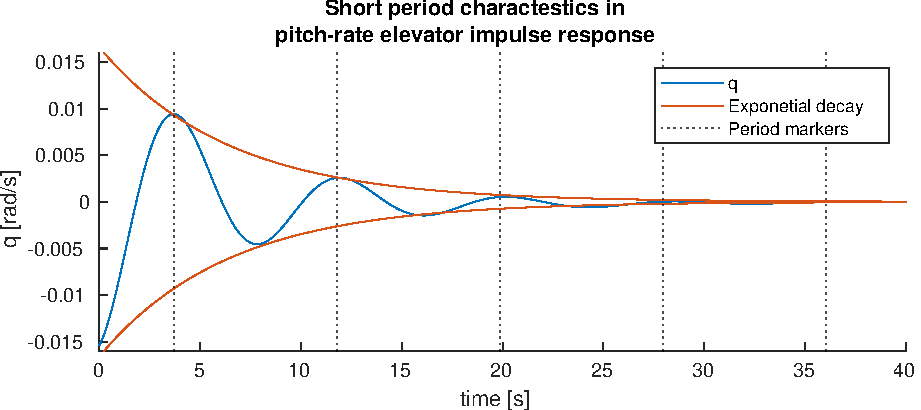
\includegraphics[width=0.6\textwidth]{figures/ol_sp}    
    \caption{Pitch-rate $q$ response during a short period oscillation, induced by a impulse elevator input.}
    \label{fig:ol_sp}
\end{figure}

\begin{figure}[ht]
    \centering
    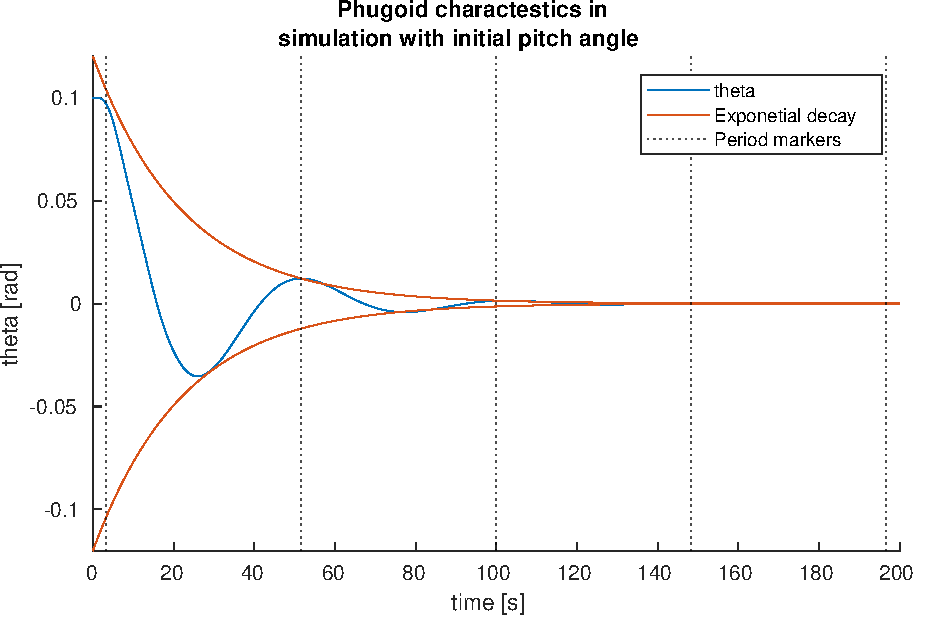
\includegraphics[width=0.6\textwidth]{figures/ol_ph}    
    \caption{Pitch angle $\theta$ response during a phugoid induced by an initial pitch angle of $\theta_0=0.1\ [rad]$}
    \label{fig:ol_ph}
\end{figure}

\subsection{Lateral motion}
Reducing the state space system such that it only contains the states $\left \{ \beta, \phi, p, r \right \}$ and inputs $\left \{ \delta_{a}, \delta_{r} \right \}$ results in the following matrices for the state space in Equation~\ref{eq:ssaclat}. $I_4$ is a 4x4 identity matrix and $0_{4,2}$ is a 4x2 zero matrix.


\begin{align*}
    A_{lat}&=\begin{bmatrix}
        -0.04905 & 0.08741 &  0.5803 & -0.8129 \\
               0 &       0 &       1 &  0.7105 \\
          -2.547 &       0 & -0.2594 &   0.151 \\
           -0.59 &       0 & 0.02607 & -0.1313
    \end{bmatrix} &
    B_{lat}&=\begin{bmatrix}
        4.181e-05 & 0.0001227 \\
                0 &         0 \\
          -0.0444 &  -0.00523 \\
         0.002184 & -0.004975 
    \end{bmatrix} \\\\
    C_{lat}&=I_4 &
    D_{lat}&=0_{4,2}
\end{align*}

\begin{align}    
    \dot{x} &= A_{lat} \cdot x + B_{lat} \cdot u_{el} \nonumber\\
    y &= C_{lat} \cdot x + D_{lat} \cdot u_{el} \label{eq:ssaclat}
\end{align}

The poles for this system are,
\begin{table}[h!]
    \centering
    \begin{tabular}{ c }
        Poles \\ \hline \hline
        $\e{-1.68}{-1}$ \\
        $\e{-1.68}{-1}$ \\
        $\e{-5.18}{-2}$ \\
        $\e{-5.18}{-2}$ \\
    \end{tabular}
    \caption{Lateral eigenmotion poles}
\end{table}

For the lateral motion is it expected to find two complex poles for the dutch roll and two real poles, one for the aperiodic roll and one for the spiral motion. However under the given flight conditions the linearization code fails and generates systems with four complex poles.

In order to continue with the assignment the flight conditions for the Accelerometer Position Analysis are used.

\begin{equation*}
    h_{apa} = 15000ft \qquad  V_{apa}=500ft/s
\end{equation*}

Linearising under these flight conditions results in the following,

\begin{align*}
    A_{lat}&=\begin{bmatrix}
        -0.2022 & 0.06414 & 0.07827 & -0.9919 \\
              0 &       0 &       1 &  0.0781 \\
         -22.92 &       0 &  -2.254 &  0.5408 \\
          6.005 &       0 & -0.0404 & -0.3146
    \end{bmatrix} &
    B_{lat}&=\begin{bmatrix}
        0.0001724 & 0.0005058 \\
                0 &         0 \\
          -0.4623 &   0.05686 \\
         -0.02437 &  -0.04687 
    \end{bmatrix} \\\\
    C_{lat}&=I_4 &
    D_{lat}&=0_{4,2}
\end{align*}

\begin{table}[h!]
    \centering
    \begin{tabular}{ r | c c c c c c }
                       & Poles                   & $\zeta$        & $\omega_n$     & $P$    & $T_{1/2}$     & $\tau$         \\ \hline \hline
        Dutch roll     & $\e{-3.20}{-1} + 2.74i$ & $\e{1.16}{-1}$ & $\e{7.77}{-1}$ & $2.28$ & $4.43$        &                \\  
                       & $\e{-3.20}{-1} - 2.74i$ & $\e{1.16}{-1}$ & $\e{7.77}{-1}$ & $2.28$ & $2.14$        &                \\ \hline
        Aperiodic roll & $2.12$                  &                &                &        & $\e{1.56}{1}$ & $\e{4.72}{-1}$ \\ \hline 
        Spiral         & $\e{-1.13}{-2}$         &                &                &        & $\e{1.56}{1}$ & $\e{8.88}{1}$
    \end{tabular}
    \caption{Lateral eigenmotions poles, damping rations, natural frequencies, periods, time to half amplitude and time constants.}
\end{table}

For the aperiodic eigenmotions, there is a new parameter $\tau$, the time constant and the time to damp to half amplitude $T_{1/2}$ is calculated differently.

\begin{align}
    \tau &= -\frac{1}{\lambda} \\
    T_{1/2} &= \ln{2}\ \tau
\end{align}

The results of these simulations are shown in the following figures. Despite being an aperiodic motions, the aperiodic roll and spiral results both contain oscillations. This is due to a less dominant dutch roll. To show this, Figure~\ref{fig:ol_apdsf} has the period markers with the period for the dutch roll added to it.

\begin{figure}[ht]
    \centering
    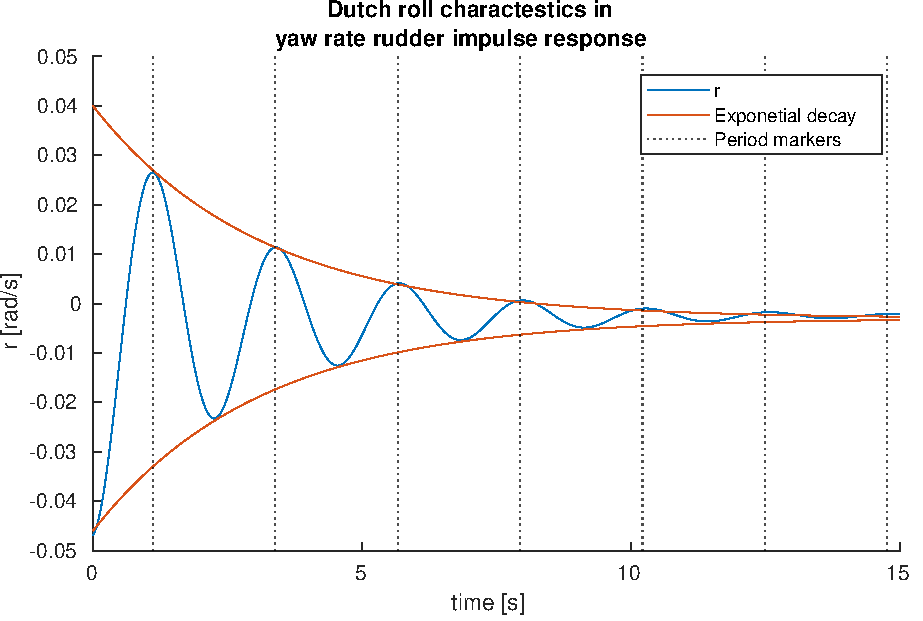
\includegraphics[width=0.6\textwidth]{figures/ol_dr}    
    \caption{Yaw rate $r$ response during a dutch roll induced by an impulse rudder input.}
    \label{fig:ol_dr}
\end{figure}

\begin{figure}[ht]
    \centering
    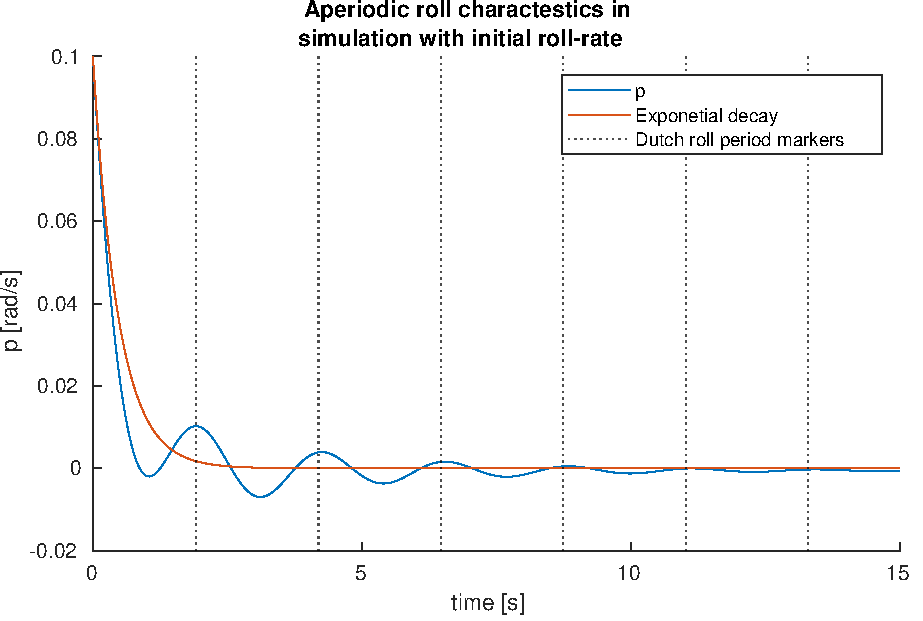
\includegraphics[width=0.6\textwidth]{figures/ol_ap}    
    \caption{Roll rate $p$ response during an aperiodic roll induced by an initial roll rate of $r_0=0.1\ 
    [rad\ s^{-1}]$}
    \label{fig:ol_apdsf}
\end{figure}

\begin{figure}[ht]
    \centering
    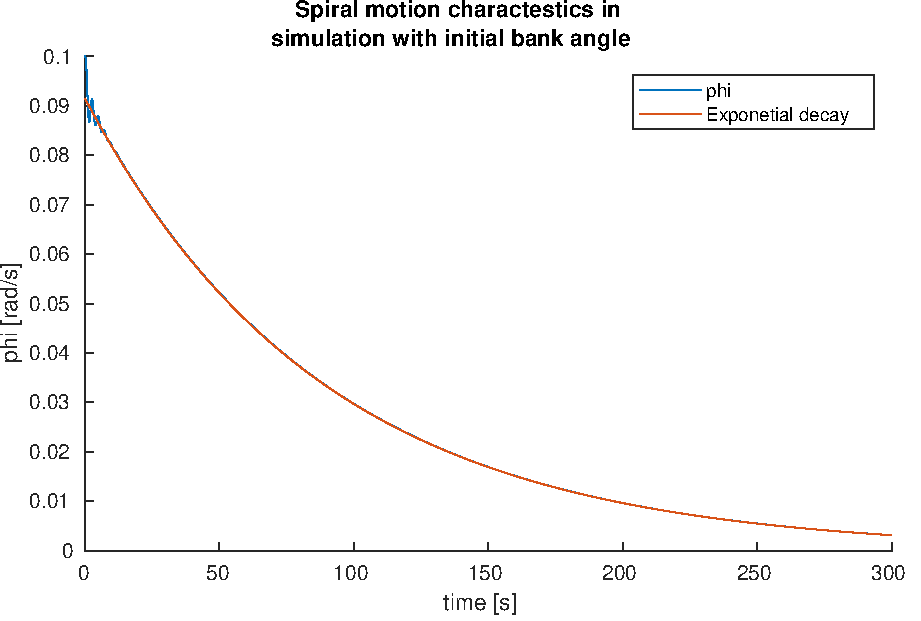
\includegraphics[width=0.6\textwidth]{figures/ol_si}    
    \caption{Bank angle $\phi$ response during a spiral motion induced by an initial bank angle of $\phi_0=0.1\ [rad]$}
    \label{fig:ol_si}
\end{figure}

\clearpage
